\def\year{2017}\relax
%File: formatting-instruction.tex
\documentclass[letterpaper]{article} %DO NOT CHANGE THIS
\usepackage{aaai17}  %Required
\usepackage{times}  %Required
\usepackage{helvet}  %Required
\usepackage{courier}  %Required
\usepackage{url}  %Required
\usepackage{graphicx}  %Required
\usepackage[ruled,vlined]{algorithm2e}
\frenchspacing  %Required
\setlength{\pdfpagewidth}{8.5in}  %Required
\setlength{\pdfpageheight}{11in}  %Required
%PDF Info Is Required:
  \pdfinfo{
/Title (Supervised Reinforcement Learning with Partial States: a Teaching Method for Action Selection for HRI)
/Author (Emmanuel Senft)}
\setcounter{secnumdepth}{0}  
 \begin{document}
% The file aaai.sty is the style file for AAAI Press 
% proceedings, working notes, and technical reports.
%
\title{Supervised Reinforcement Learning with Partial States: \\
 a Teaching Method for Action Selection for HRI}

\author{Emmanuel Senft \\
CNRS \\
Plymouth University \\
United Kingdom\\
\And S\'{e}verin Lemaignan\\
CNRS \\
Plymouth University \\
United Kingdom\\
\And Paul Baxter\\
L-CAS\\
University of Lincoln\\
United Kingdom\\
 \And Tony Belpaeme\\
 CNRS\\ Plymouth University (UK) \\ iMinds \\ Ghent University (Be)}

\maketitle
\begin{abstract}
As robots will integrate human society, they will have to satify humans'
expectations. However at the design time, it seems hardly possible to
know in advance exactly all the behaviours expected from the robot. As such to
be accepted in human society robots have to learn how to interact with humans.
But learning social interaction is a complex task. Firstly, no simulator of
human interactions precise enough exists today, so the learning will probably have
to be made online and in the real world.
This means that robots will have to learn directly from interacting with humans,
which limits the quantity of datapoint possible to gather and make exploration
riskier as actions will have real impacts on humans or the robot itself. Additionally,
no clear reward function exists for social interactions. As such we argue that
robots will highly profit from human expertise and guidance to learn social
interactions. And as the quantity of data is limited, they also will have to make the most out of each datapoint. We
propose to combine the Supervised Progressively Autonomous Robot Competencies
allowing a safer online learning and Reinforcement Learning based on partial
states rather than full states to accelerate the learning by using more
information form the human teacher.
\end{abstract}
%===============================================================================

\section{Introduction}

Human-Robot Interaction (HRI) aims at having humans and robot living together
in the society, interacting socially in many different environments and
contexts. Robot are expected to behave appropriately regardless of the domain
of interaction. However, not all behaviours can be known in advance and be
implemented in the robot before its deployment in the real world. Similarly to
 humans, robots need
to be able to learn new tasks, new actions policies, new social norms and how
to make sense of the world surrounding them.

When interacting in the real world, humans face huge spaces of almost unlimited
dimensions, and despite this complexity, humans, and especially children are able
to learn quickly, often from only a few demonstrations or examples. One of the
 reason could be that they are able to take the most out of every datapoint available to them. 
 On the other
hand, recent impressive advances in Machine Learning such as Deep Learning~\cite{lecun2015deep}
have been made possible by the availability of huge dataset covering millions
of labeled examples or dozens of hours of recording. These progress have
targetting either perception, where labeled datapoints can be available or
action selection in virtual environments where the impact of actions is
limited.

However, these immense labelled dataset or virtula worlds are not existent for
social interaction. To learn how to interact with humans, robots will have to
experiment in the real world facing real reactions from their actions. So they
have to learn quickly while consistently exhibiting a decent behaviours.
One way of ensuring this correct  behaviours is to use a human to supervised the
the robot during the early phase of learning, and this human can also provide
inputs to boostrap the learning, achieving a faster learning. This paper present
a novel method based on human supervision, feature highlighting and partial
state reinforcement learning to achieve this fast and safe learning.

%===============================================================================

\section{Background}
\subsection{Reinforcement Learning}

The main framework to provide a robot with autonomous learning is Reinforcement
Learning (RL)~\cite{kober2013reinforcement,sutton1998reinforcement}. In RL, an
agent is interacting in an environment
providing numerical reward in reaction to the agent's actions and
the agent learns an action policy to maximise the expected cummulative discounted
reward obtained by the agent.

Classic approaches RL generally rely on exploring virtual environments where the agent
tries to maximise the reward. In most of the cases where RL achieves success, it
had access to a virtual environment where the only real cost of exploring is
time and energy, and the agent can interact as long as needed to gather
enough information on the environment to find a correct action policy. When
these conditions are reunited, RL can achieve impressive results, as shown by
the victory of a computer in Backgammon back in the 90s~\cite{tesauro1995temporal} or more recently the success achieved in playing
Atari games based only on the image and the game rewards~\cite{mnih2015human}.

\subsection{Human enhanced Reinforcement Learning}

No simulator of world, and especially of social interactions allows robots to 
learn in a virtual environment, so robots, especially if the have to interact
with humans have to be able to learn in the real world.
However, in the real physical world, every actions have an impact on the
environment, especially in HRI when actions can upset and negatively impact
humans interacting with the robot. Additionally acquiring datapoints in can be
expensive in term of time and other ressources. As such many approaches aiming
at providing robot with learn to interact in the real world have relied on
knowledge provided by a human in different way to avoid this random exploration
presenting risk to the robot and persons interacting with it.

\subsubsection{Initial knowledge}
One way to use human knowledge to help an agent to learn is through providing
initial knowledge. By providing demonstrations of an expected actions policy,
humans can boostrap the learning and provide the agent with a more appropriate
action policy that it can improve over time. 

These demonstrations can be used to create an initial action policy which could
have been discovered autonomously, but without requiring an initial discovery
phase where the performance has to be low when the agent is learning from its
environment. Recent work~\cite{hester2017learning} have shown that using initial
human demonstrations can allow the initial performance to be much better than
starting from scratch in playing Atari games, and even sometimes this allow to
achieve higher performance than only relying on exploration to learn an action
policy.

In some cases, the state space is too big to rely only on random exploration to
reach a successful action policy. For example the game of Go in its larger board
size contains more than $10^{210}$ states, so exhaustive search is not possible
with today's ressources. Authors of \cite{silver2016mastering} started with
supervised learning from go master's games to learn a decent policy and then
used deep learning, self play and tree search to achieve super-human
capabilities and beatting humans best players.

Another way to use these demonstrations is Inverse
Reinforcement Learning, the agent derives from demonstrations of an expert an
expected reward function that it can use to improve a policy based on the
demonstrations and so achieving higher performance than the demonstrations
themselves. By using this technic, Abbeel managed to teach an autonomous
helicopter to do high level acrobatics often only executable by high level
expert~\cite{abbeel2004apprenticeship}. 

%One of the main challenge when applying RL to robotics is poor perfermance in
%the early stages of the learning as the agent has to explore the environment to
%gather initial knowledge. This challenge is especially
%important for robotics as trials often have to happen in the real world (as
%simulator close enough to the real world as not available) and as such can
%present risks for the robot or for the persons interacting with it. 

\subsubsection{Guiding the learning}
Rather than solely providing initial knowledge to the agents, humans can also guide the
agent throughout the learning in a more human-like teaching scenario. 

A first possibility is organising the tasks the robot will face. 
This approach, known as scaffolding \cite{saunders2006teaching} progressively
increase the difficulty and complexity of the task or the environment as the
robot is learning to achieved complex policy not directly learnable in the final
environment.

Another possibility is shaping. For example, the TAMER framework
\cite{knox2009interactively}, allows to teach an agent an action policy in an
environment providing no rewards using a human observer to supply rewards to the
agent. One of the interest of this approach is that the teacher can adapt the
rewards to the current policy of the agent, for example starting to reward
positively suboptimal behaviours but which still improve the current policy and
later, as the agent improve its behaviour reward these same suboptimal behaviour
negatively and only the optimal ones positively.

A last possibility to guide the the learning is to bias the action selction.
In~\cite{thomaz2008teachable}, the authors propose to use a human supervisor to
supply  an agent both rewards and potential guidance or advise indicating where
the agent should pay attention, or what it should do next. And they show that
giving the power to the supervisor to bias the action selection can improve the
learning, making it faster, safer.

%===============================================================================

\section{Proposition}
\subsection{Supervised Progressively Autonomous Robot Competencies}

As a way to enable a human supervisor to teach a robot an action policy while
interacting with its environment, we proposed the Supervised Progressively
Autonomous Robot Competencies (SPARC) in~\cite{senft2015sparc}. SPARC defines an
interaction dynamic between an agent learning an action policy while interacting
in an environment and a
supervisor teaching this agent what to do. The main goal of SPARC is
enabling a robot to learn from a supervisor while ensuring that every action
executed by the robot has approval of the supervisor but without requiring this
supervisor to manually enforce every single action.

The main concept in SPARC is giving the supervisor the control over the agent
action and combine this with online learning on the agent side. This control is
achieved using a suggestion/correction mechanism whereby the agent presents
to the supervisor the action about to be executed and the supervisor can cancel
this action before its execution or not doing anything, letting the action being
executed after a delay. Additionally, the supervisor can select actions to be
executed by the agent. The actions selected, accepted or canceled by the supervisor can be
used as input with the current state by a learning algorithm to progressively
improve the future suggestions thus reducing the reliance on the supervisors.

Giving power to an expert to correct the actions of the agent before the
execution can ensure that even in the early phases of the learning the agent can
have an appropriate action policy for the current environment as shown in
Figure~\ref{fig:comparison} while making the learning faster compared to
autonomous learning. (update figure with autonomous learning, classical learning from human rewards
and sparc)

\begin{figure}
    \centering
    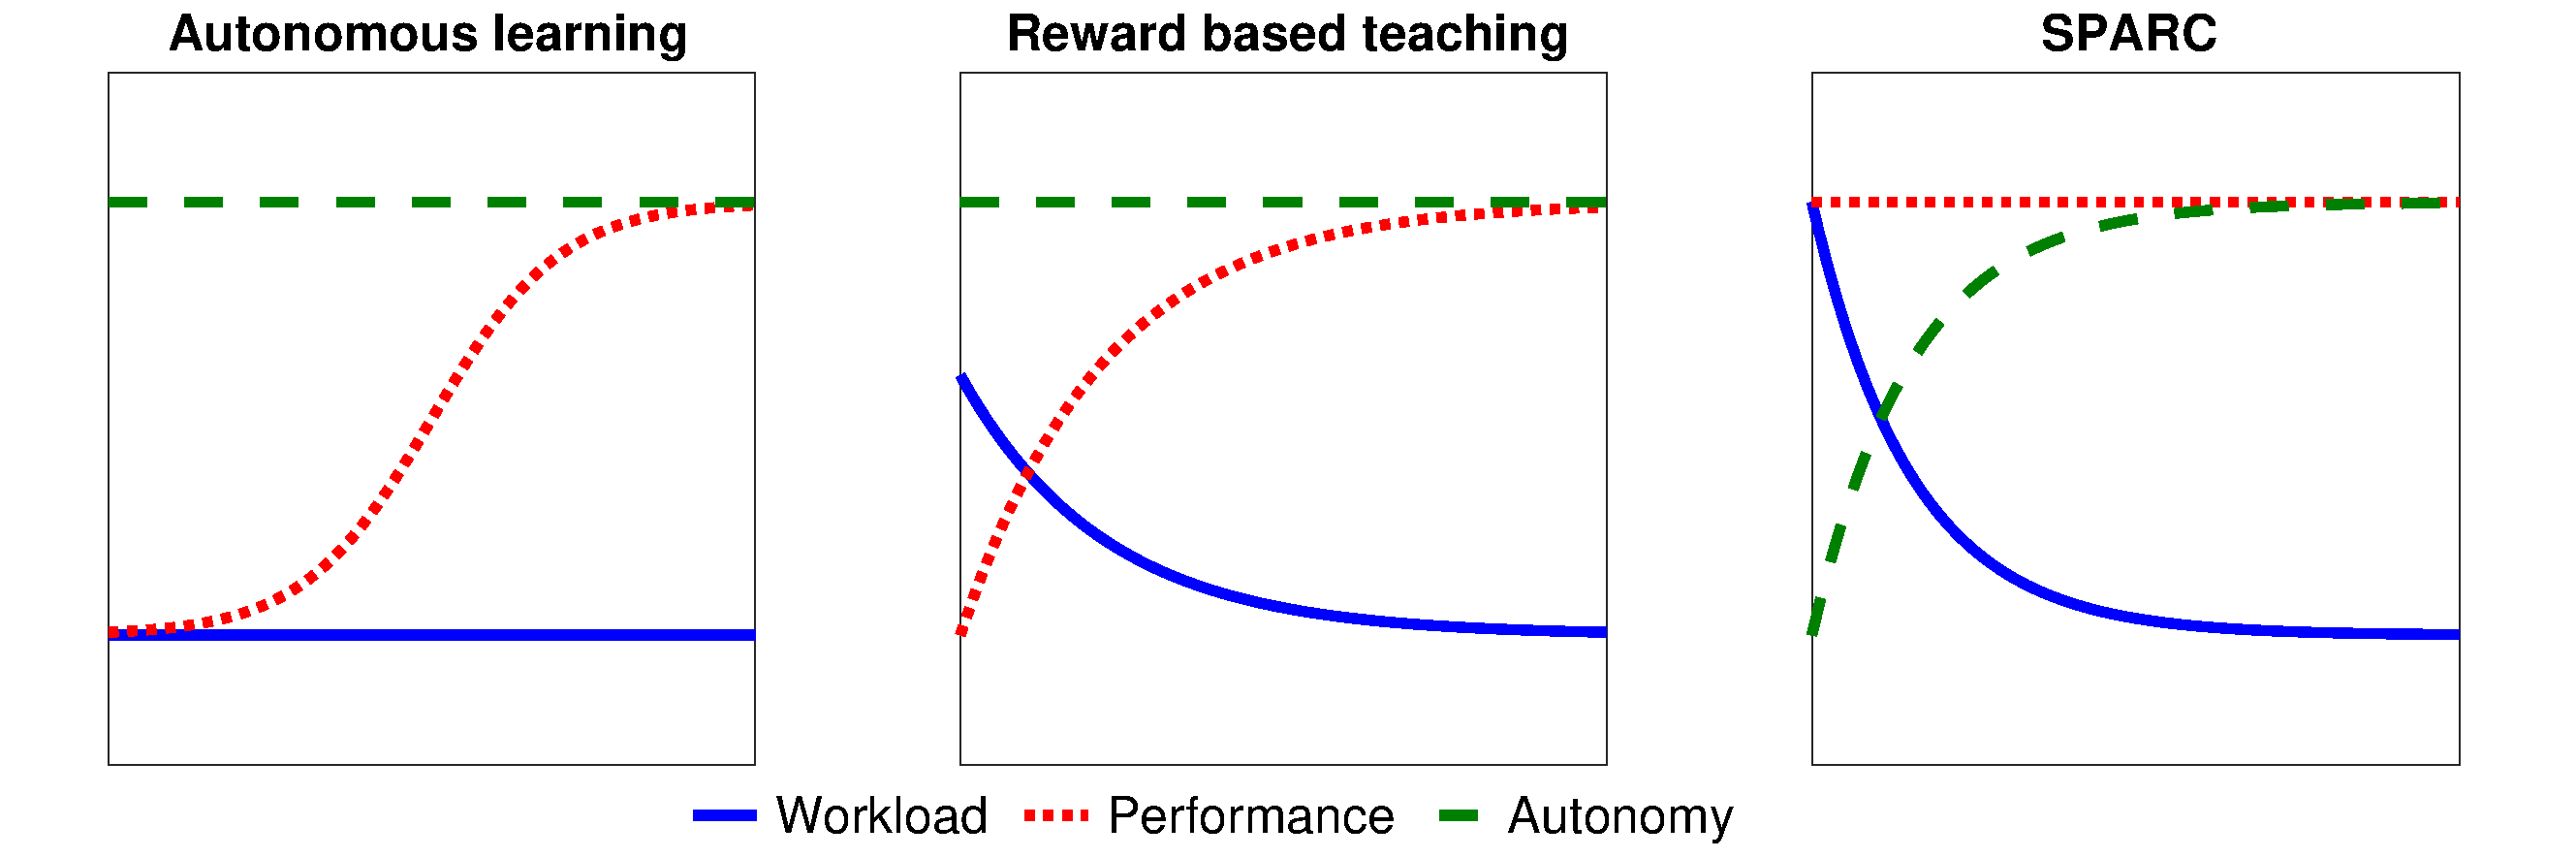
\includegraphics[width=0.9\linewidth]{./fig/motivation.pdf}
    \caption{Idealised expectation for performance, autonomy and human workload for a
    an autonomous learner, an approach using human rewards and SPARC.}
    \label{fig:comparison}
\end{figure}

SPARC has been design with the idea of teaching a robot to interact with humans,
it is specially usefull when the frequency of action selection is low (less than
1Hz) so action can be evaluated by a human before being executed, when the agent
has to learn with a limited number of datapoints and when
undesired actions executed by an agent can have a high cost and are to be
avoided. 

In \cite{senft2017supervised}, we presented a way to combine SPARC and RL, by
assigning a positive reward to every action executed by the robot as it would
have been passively or actvely validated by the supervisor. However this method
was not making use of any type of generalisation, it was directly mapping a
single state action pair to a reward, and as such had limited efficiency in
environments with a continuous or high dimensional space or undeterministic
transition from one state to another.

\subsection{Partial-State Supervised Reinforcement Learning}

Humans evolve in a highly complex environment with a nearly infinite number of
dimensions originating from different modality through our senses. But, despite
this complexity, we can select actions according to important features of the
state, regardless of other parts of it.

Taking inspiration from this observation, we argue that focusing on partial states, rather
than full states can both increase the speed of learning for an agent and
provide some of the generalisation required to interact in complex environment.
Guidance from a human can highlight important features in the state space and
associate them to actions. This shifts the state action pair paradigm to a
partial-state action pair, and in the case of RL, the tuple: partial-state,
action and reward. 



%A classical approach to generalise in RL is to use a first layer of neural
%network or to use deep reinforcement learning which relies on deep neural
%networks to learn a mapping state action Qvalue for example. (ADDREF)
%These approaches, neural network based, relies on having a large number of
%datapoints to converge toward a good function approximator. However, as
%discussed previously, in many application, these amounts of data are not
%possible to be obtained and a robot might need to adapt to different persons and
%be retrained quickly.

%With that idea in mind, we propose to make a better use of human inputs, and ask
%the supervisor to identify which features of the environment are linked to the
%current selected action.

%===============================================================================
\section{Methodology}

\subsection{Supervisation}
Similarly to a SPARC setup, the supervisor can select actions, or when presented
with an action about to be executed by the robot either cancel it or let
it be executed.

In addition to these actions, the supervisor can use the GUI to select features
of the environment that can be sent to the algorithm to reduce the state associated
to this action to a partial-state. Similarly, the algorithm can indicate which
parts of the states have been used for the selection to the supervisor who can
correct them while the action is being executed.

%Example?

\subsection{Learning algorithm}

In a first approach, the presence of an expert supervisor who can evaluate the
expected future impacts of an action removes the problem of credit assignment
for delayed rewards and allows us to consider only a myopic approach. 

For this paper, we will reuse the formalism of rewardless Markov Decision 
Process to identify the different elements of our system. The agent has action
to a set of actions A, a state S (represented as a vector of n dimensions of
values $\in [0;1]$). With each dimension of S representing features in the
environment.

At the state $s_{t}$ the agent receives the action $a_{i}$ with the partial
state $s'$ defined in a subspace $S' \subseteq S$ (defined by selecting only a
number $n' \leq n$ of the dimensions of S). For example, a state s could be
defined in 4 dimensions such as ${s=[1,0.2,0,0.5]}$, and s' in two dimensions with
${s'=[-,0.2,0,-]}$ with symbol '$-$' reprensenting the dimensions removed.

We store in memory the partial-state action pair $s'$-$a_{i}$, with the reward 1
as the action has been selected by the supervisor. Similarly, if an action has
been canceled by the supervisor, the partial-state action pair will be assigned to a
reward -1.

After interacting with the system under the supervisors control, the actions
will have associated to each action ${a \in A}$, a collection $C_{a}$ of pairs
partial-state reward. When facing a new state $s$ where an action has to be
selected, the agent can select an action following Algorithm \ref{algo}.

\begin{algorithm}
    \DontPrintSemicolon
    \SetKwInOut{Input}{inputs}\SetKwInOut{Output}{output}
    \Input{Current state s, action-partial state rewards tuples}
    \Output{selected action $\pi(s)$}
    \ForEach{a $\in$ A}{
        \ForEach{s'-r $\in C_{a}$}{
            compute similarity
            $\Delta(s',s)=1-\frac{\sum_{i}^{n'}(s'(i)-s(i))^{2}}{n'}$
        }
        $\Delta(a)=max(\Delta)$

        $r(a)=R(argmax_{s'} \Delta(s'))$
    }
    $\pi(s) = argmax_{a}\Delta(a) \cdot r(a)$

    \caption{Algorithm for selecting an action based on previous
    partial-state action rewards tuples and current state}
    \label{algo}
\end{algorithm}
In case of mutiple states s' with different rewards, only the most recent one
can be stored in memory, allowing a supervisor to correct potential errors, or
adapt to change of desired policy.

When proposing an action following Algorithm~\ref{algo}, the agent can also use
the dimensions of the similar state s' used for the selection to indicate the
supervisor which parts of the state have been used for the action selection.

%===============================================================================
\section{Challenges}

A large body of the
Interactive Machine Learning research is focused on simple inputs from the
humans, such as providing labels \cite{cakmak2012designing}, rewards
\cite{knox2009interactively} or kinesthetic demonstrations
\cite{billard2008robot}. However, as stated in \cite{amershi2014power}: "people
want to demonstrate how learners should behave" and "users may desire richer
control over machine-learning systems than simply labeling data". Human teachers
want to be more active and involved in the teaching process, to make their
student learning faster. 
And, as shown in \cite{senft2017supervised}, providing teacher with this control
can keep the agent in relevant states of the environment, speeding the learning
and reducing the risk to have the robot execute undesired actions.

In human social learning, both interactants have access to a similar set of
inputs: the senses available to a human body, and the teacher has additional
knowledge about the environment that can be communicated in an open ended way to
the learner. On the other in human-robot teaching, the way to sense the world
can be highly different between the two partners, and as of today, there is no
open ended way of communicating new concepts or explication as natural langage
processing is not yet solve. This creates two main challenges to make robot
learning for human use complex inputs: 
\begin{itemize}
    \item Having a mapping between the action state space of the human and the
            robot ensuring that feature used for action selection for one
            interactant are available to the other.
    \item Communicating these features from one participant to the other: allow
        the robot to make sense of the human's instructions and the human to
        understand the robot's intentions.
\end{itemize}

\section{Future work}

This method still has to be tested in a real Human-Robot Interaction, and this
evaluation is currently being implemented and will be tested in a near future.

Other way of extending the current work would be to combine it with the
possibility of letting the agent continue to explore in the absence of a
supervisor around a learnt action policy to keep improving its behaviour. This
could be done by allowing the supervisor to provide rewards during the learning
phase, rewards which could also be assigned to partial states. The system could
also learn to predict these rewards in an approach similar to TAMER 
\cite{knox2009interactively}. But in the case of an absence of supervisor, the assumption that only a
myopic action selection is sufficient would not hold anymore and the problem of
delayed rewards would have to be tackled. It could be for example possible to
adapt well known algorithms such as QLearning to handle partial states rather
the full states.

%===============================================================================
\section{Conclusion}
\label{sec:conclusion}
%==============================================================================
\section{Acknowledgments}
This work was supported by the EU FP7 DREAM project (grant no.  611391) and EU
H2020 Marie Sklodowska-Curie Actions project DoRoThy (grant 657227).  

\bibliographystyle{aaai} \bibliography{biblio}
\end{document}
